% ========================================================================================================
\clearpage
\subsection{Flow past a rotating disk}\label{sec:pillInBoxFlow}


{%%%%%%%%%%
% 
\newcommand{\figWithCaption}[5]{
\begin{scope}[yshift=#1cm]
  \draw ( 0.0,0.0) node[anchor=south west,xshift=-4pt,yshift=+0pt] {\trimfiga{#2}{\figWidtha}};
  \draw ( 8.0,.0) node[anchor=south west,xshift=-4pt,yshift=+0pt] {\trimfiga{#3}{\figWidtha}};
  \draw ( 0.0,0.3 ) node[draw,fill=white,anchor=south west,xshift=+1pt,yshift=-4pt] {\scriptsize #4};
  \draw ( 8.0,0.3 ) node[draw,fill=white,anchor=south west,xshift=+1pt,yshift=-4pt] {\scriptsize #5};
\end{scope}
}% end figWithCaption
\newcommand{\figWidtha}{6.0cm}
\newcommand{\trimfiga}[2]{\trimPlotb{#1}{#2}{.0}{.0}{.05}{.1}}
% 
\newcommand{\figWidthb}{5.5cm}
\newcommand{\trimfigb}[2]{\trimPlotb{#1}{#2}{.05}{.05}{.05}{.1}}
\newcommand{\figWidthc}{6cm}
\newcommand{\trimfigc}[2]{\trimPlotb{#1}{#2}{.025}{.025}{.095}{.095}}
% % -----------------------------------------------------------------------------------------------------------------------------------------
\begin{figure}[hbt]
\begin{center}
\begin{tikzpicture}[scale=1]
  \useasboundingbox (0,.75) rectangle (16.,21.25);  % set the bounding box (so we have less surrounding white space)
%
\draw (0.0,15.75)  node[anchor=south west,xshift=-4pt,yshift=+0pt] {\trimfigc{\cgDoc/ins/fig/pillInABoxGrid}{\figWidthc}};
\draw (8.0,15.75)  node[anchor=south west,xshift=-4pt,yshift=+0pt] {\trimfigb{\cgDoc/ins/fig/pillInABoxGridZoom}{\figWidthb}};
%
\figWithCaption{10.5}{\cgDoc/ins/fig/pillO4G8t1}{\cgDoc/ins/fig/pillO4G8t3}{$t=1$ (1/8 rotation)}{$t=3$ (3/8 rotations)}
\figWithCaption{5.25}{\cgDoc/ins/fig/pillO4G8t5}{\cgDoc/ins/fig/pillO4G8t11}{$t=5$ (5/8 rotations)}{$t=11$ (1 3/8 rotations)}
\figWithCaption{0}{\cgDoc/ins/fig/pillO4G8t13}{\cgDoc/ins/fig/pillO4G8t14}{$t=12$ (1 5/8 rotations)}{$t=14$ (1 6/8 rotations)}
%
 % \draw (current bounding box.south west) rectangle (current bounding box.north east);
% grid:
%\draw[step=1cm,gray] (0,0) grid (16,21.);
\end{tikzpicture}
\end{center}
 \caption{Flow past a rotating {\em disk} in channel. Top: Overlapping grid, $\Gc^{(2)}$ (second-order), for the disk and channel. 
   Contour plots of the enstrophy (max contour $\xi=40$) on grid $\Gc^{(8)}$, using the fourth-order accurate scheme AFS42. }
  \label{fig:pillInBoxFlow}
\end{figure}
% -----------------------------------------------------------------------------------------------------------------------------------------------
%
}%%%%%%%%%%%%


We simulate the flow past a rotating {\em disk} (``pill'' or ``coin'').
The grid for this problem was generated from the ogen command file {\tt pillInABoxGrid.cmd}.
The solution was computed with the Cgins command file {\tt cg/ins/cmd/pillInABox.cmd}.
The geometry for the problem, as shown in Figure~\ref{fig:pillInBoxFlow},
consists of disk (``pill'') shaped body. The edge of the disk is  constructed from a body of revolution 
using a cross-section defined by a smooth-polygon.
The disk is embedded in a channel. A refinement patch is located near the disk. A coarser background grid
covers the majority of the channel.
Let $\Gc^{(j)}$ denote the composite grid for this geometry. The target grid spacing is $\ds=1/(10 j)$.
The grid spacing is stretched in the normal direction to the body so that the boundary layer
spacing is $\dsbl$. 


% movie: pillO4G8.mpg  G8: 5.7M pts, 5 restarts required but code was hanging in HDF
% submit.p -jobName="pill" -bank=windpowr -out="pillO4G8b.out" -walltime=16:00 -submit=0 -cmd='srun -N2 -n32 -ppbatch $cginsp -noplot pillInABox -g=pillInABoxGride8.order4.ml4 -nu=1.e-4 -tp=.02 -tf=10. -move=1 -freq=.125 -cfl=3. -slowStartCFL=2. -slowStartSteps=100 -slowStartRecomputeDt=10 -recomputeDt=50 -psolver=mg -ts=afs -ad2=0 -ad4=1 -freqFullUpdate=1 -debug=1 -numberOfParallelGhost=4 -project=0 -restart="/p/lscratchd/henshaw/runs/cgins/pillInABox/pillO4G8a.show" -show=pillO4G8b.show -go=go'

Figure~\ref{fig:pillInBoxFlow} shows the solution on grid $\Gc^{(8)}$ ($7$M pts). 
The incoming flow is in the $x$-direction with $u=1$.
Contours of the enstrophy $\xi$, (magnitude of the vorticity vector, $\xi=\| \grad\times \uv\|$) are shown
with the maximum contour level set at $\xi=40$. 
The solution was computed with the scheme AFS4 and the SSLES4 turbulence model ($\nu=10^{-4}$). 


Figure~\ref{fig:pillInBoxFlow16} shows the solution on the finer grid $\Gc^{(16)}$ ($51$M pts).

{%%%%%%%%%%
% 
\newcommand{\figWithCaption}[5]{
\begin{scope}[yshift=#1cm]
  \draw ( 0.0,0.0) node[anchor=south west,xshift=-4pt,yshift=+0pt] {\trimfiga{#2}{\figWidtha}};
  \draw ( 8.0,.0) node[anchor=south west,xshift=-4pt,yshift=+0pt] {\trimfiga{#3}{\figWidtha}};
  \draw ( 0.0,0.3 ) node[draw,fill=white,anchor=south west,xshift=+1pt,yshift=-4pt] {\scriptsize #4};
  \draw ( 8.0,0.3 ) node[draw,fill=white,anchor=south west,xshift=+1pt,yshift=-4pt] {\scriptsize #5};
\end{scope}
}% end figWithCaption
\newcommand{\figWidtha}{6.0cm}
\newcommand{\trimfiga}[2]{\trimPlotb{#1}{#2}{.0}{.0}{.05}{.1}}
% 
\newcommand{\figWidthb}{5.5cm}
\newcommand{\trimfigb}[2]{\trimPlotb{#1}{#2}{.05}{.05}{.05}{.1}}
\newcommand{\figWidthc}{6cm}
\newcommand{\trimfigc}[2]{\trimPlotb{#1}{#2}{.025}{.025}{.095}{.095}}
% % -----------------------------------------------------------------------------------------------------------------------------------------
\begin{figure}[hbt]
\begin{center}
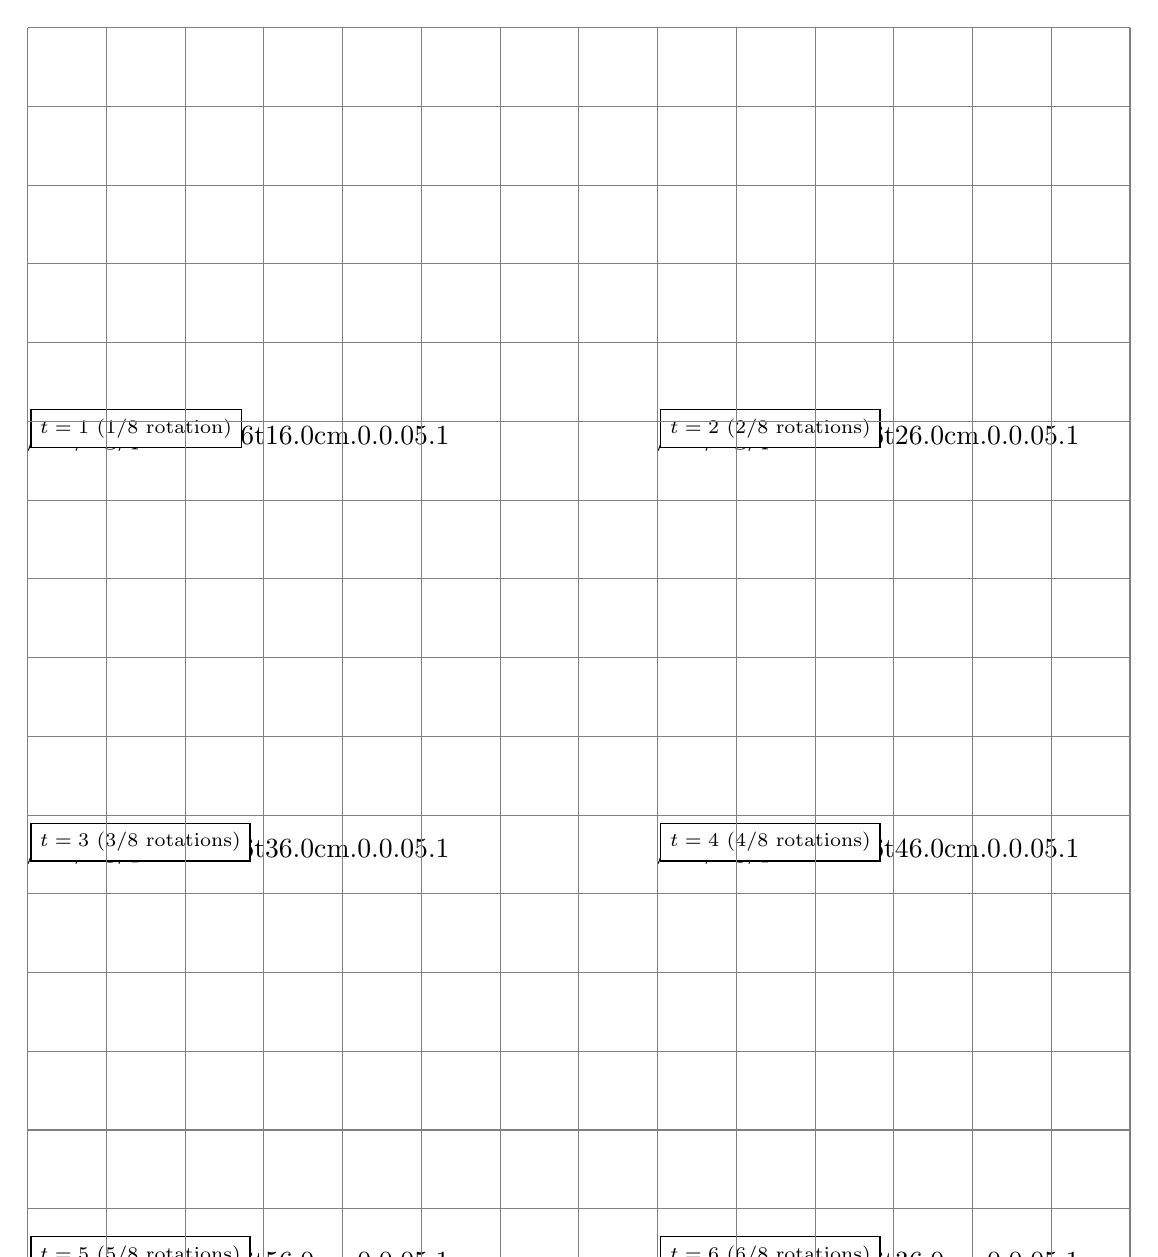
\begin{tikzpicture}[scale=1]
  \useasboundingbox (0,.75) rectangle (14.,16.0);  % set the bounding box (so we have less surrounding white space)
%
\figWithCaption{10.5}{\cgDoc/ins/fig/pillO4G16t1}{\cgDoc/ins/fig/pillO4G16t2}{$t=1$ (1/8 rotation)}{$t=2$ (2/8 rotations)}
\figWithCaption{5.25}{\cgDoc/ins/fig/pillO4G16t3}{\cgDoc/ins/fig/pillO4G16t4}{$t=3$ (3/8 rotations)}{$t=4$ (4/8 rotations)}
\figWithCaption{0}{\cgDoc/ins/fig/pillO4G16t5}{\cgDoc/ins/fig/pillO4G16t3}{$t=5$ (5/8 rotations)}{$t=6$ (6/8 rotations)}
%
 % \draw (current bounding box.south west) rectangle (current bounding box.north east);
% grid:
\draw[step=1cm,gray] (0,0) grid (14,16);
\end{tikzpicture}
\end{center}
 \caption{FINISH ME. Flow past a rotating {\em disk} in channel. 
   Contour plots of the enstrophy (max contour $\xi=50$) on grid $\Gc^{(16)}$, using the fourth-order accurate scheme AFS42. }
  \label{fig:pillInBoxFlow16}
\end{figure}
% -----------------------------------------------------------------------------------------------------------------------------------------------
%
}%%%%%%%%%%%%


\endinput